\documentclass[pdf]{beamer}
\usepackage[utf8]{inputenc}
\usepackage[estonian]{babel}
\usepackage{eurosym}

\usetheme{Madrid}
\setbeamertemplate{navigation symbols}{}

\title[Alglaadur ESTCube-1 kahele moodulile]{Alglaadur ESTCube-1 käsu- ja andmehaldussüsteemile ja kaameramoodulile}
\author{Karl Tarbe}

\begin{document}

\begin{frame}[plain]
	\titlepage
\end{frame}

\section{Sissejuhatus}
\begin{frame}{Toetus}
	\center{
\includegraphics[width=0.9\textwidth]{ITA-logo.jpg}}
\end{frame}
\begin{frame}{Estcube-1}
	\begin{columns}
		\begin{column}{0.5\textwidth}
			\begin{itemize}
				\item 2008, suvi
				\item \(10 \times 10 \times 10\) cm\({}^3\)
				\item 1.048 kg
				\item 670 km
				\item 100 000 \euro
			\end{itemize}
		\end{column}
		\begin{column}{0.5\textwidth}
			\center{
\includegraphics[width=\textwidth]{estcube-logo.png}}
		\end{column}
	\end{columns}
\end{frame}

\begin{frame}{Estcube-1}
	\begin{columns}
		\begin{column}{0.5\textwidth}
			\center{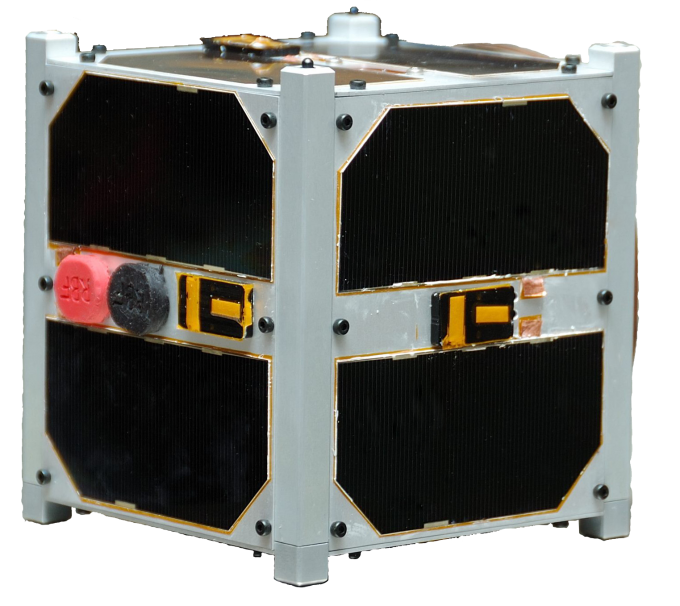
\includegraphics[width=\textwidth]{estcube-photo.png}}
		\end{column}
		\begin{column}{0.5\textwidth}
			\center{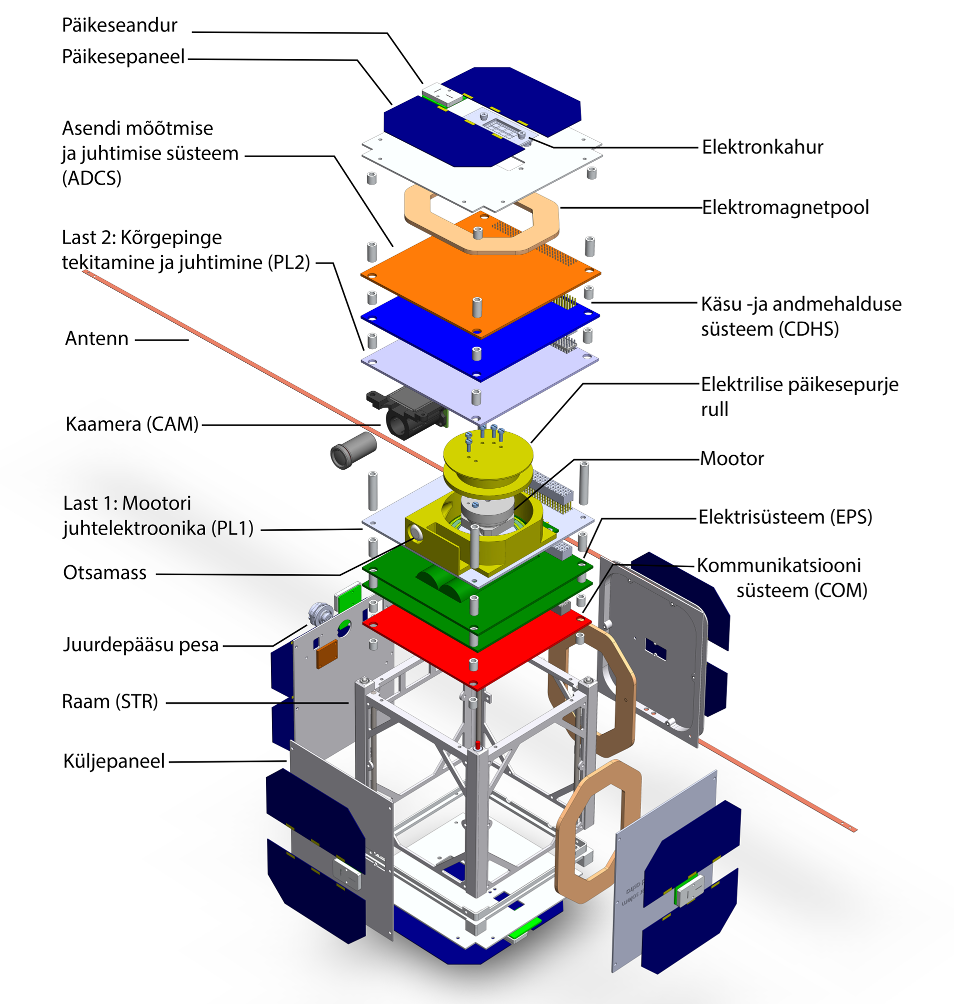
\includegraphics[width=\textwidth]{estcube-assembly.png}}
		\end{column}
	\end{columns}
\end{frame}

\begin{frame}{Käsu- ja andmehaldussüsteem (CDHS)}
	\begin{columns}
		\begin{column}{0.5\textwidth}
			\begin{itemize}
				\item \textit{Command and Data Handling System} \(\to\) CDHS
				\item STM32F103 mikrokontroller
				\item Riistvaraline dubleeritus
				\item FRAM mälud
			\end{itemize}
		\end{column}
		\begin{column}{0.5\textwidth}
			\center{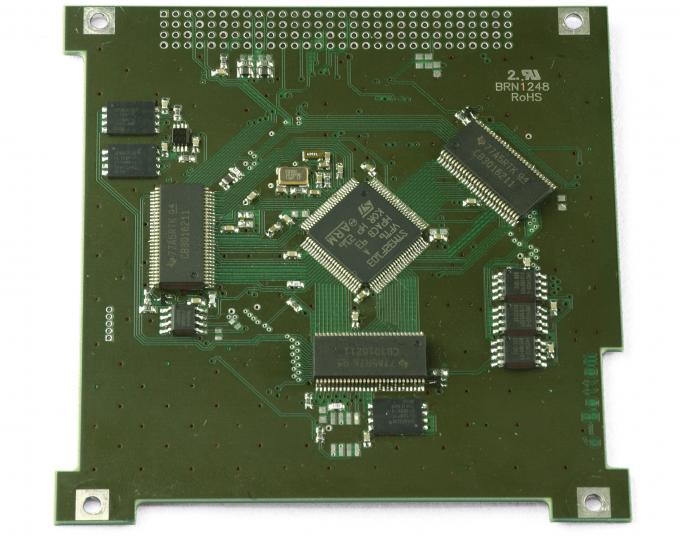
\includegraphics[width=\textwidth]{estcube-CDHS.jpg}}
		\end{column}
	\end{columns}
\end{frame}

\begin{frame}{Kaameramoodul (CAM)}
	\begin{columns}
		\begin{column}{0.5\textwidth}
			\begin{itemize}
				\item STM32F217 mikrokontroller
				\item 640\(\times\)480 
				\item FRAM mälu
			\end{itemize}
		\end{column}
		\begin{column}{0.5\textwidth}
			\center{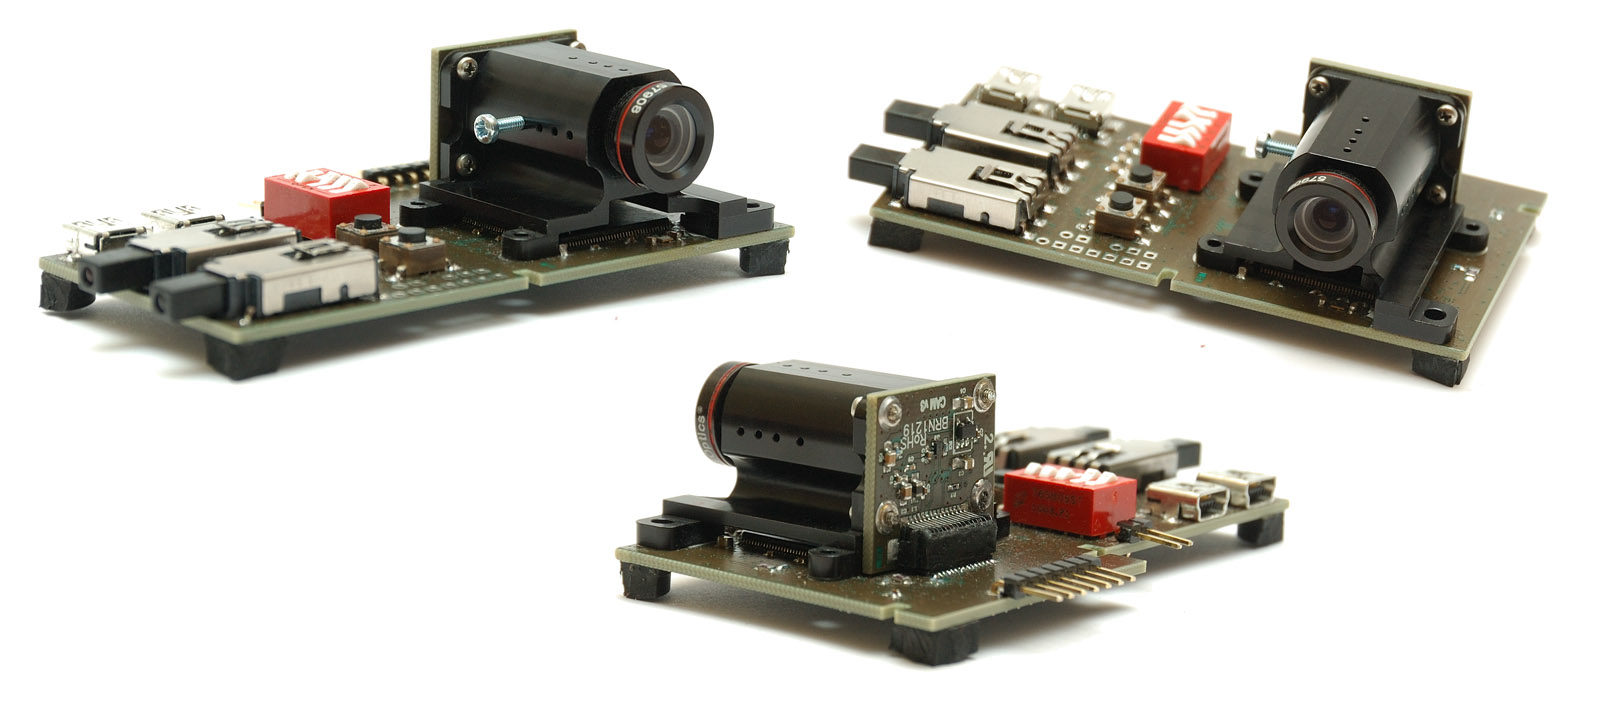
\includegraphics[width=\textwidth]{estcube-CAM.jpg}}
		\end{column}
	\end{columns}
\end{frame}

\section{Alglaadimine}
\begin{frame}{Alglaadur}
	\begin{block}{Ülesanded}
		\begin{itemize}
			\item Tarkvara terviklikkuse kontrollimine
			\item Tarkvara kopeerimine välimisest mälust sisemisse
			\item Põhitarkvara käivitamine
			\item Tegevuste logi salvestamine
		\end{itemize}
	\end{block}
	\begin{block}{,,Kasutajaliides''}
		\begin{itemize}
			\item Alglaadurile käskude andmine
			\item Tegevuste logi lugemine
		\end{itemize}
	\end{block}
\end{frame}

\begin{frame}{Mälud}
	\begin{columns}[t]
		\begin{column}{0.46\textwidth}
			\begin{block}{FLASH}
				\begin{itemize}
					\item Asub mikrokontrolleri sees.
					\item Saab muuta lehe kaupa.
				\end{itemize}
			\end{block}
		\end{column}
		\begin{column}{0.46\textwidth}
			\begin{block}{\textit{Ferroelectric RAM} (FRAM)}
				\begin{itemize}
					\item Ei asu mikrokontrolleris.
					\item Saab muuta baidi kaupa.
				\end{itemize}
				Juurdepääs on üle SPI või I\({}^2\)C siini.
			\end{block}
		\end{column}
	\end{columns}
\end{frame}

\begin{frame}{SPI ja I\({}^2\)C}
	\begin{columns}
		\begin{column}{0.46\textwidth}
			\begin{block}{\textit{Serial Peripheral Interface}}
				\center{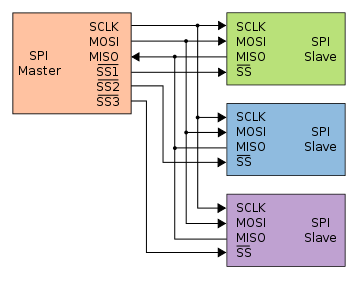
\includegraphics[width=\textwidth]{SPI.png}}
			\end{block}
		\end{column}
		\begin{column}{0.46\textwidth}
			\begin{block}{\textit{Inter-Integrated Circuit}}
				\center{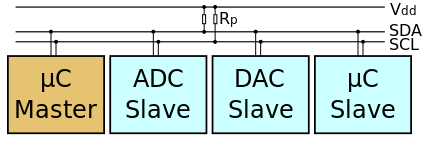
\includegraphics[width=\textwidth]{I2C.png}}
			\end{block}
		\end{column}
	\end{columns}
\end{frame}

\begin{frame}{Tarkvara tervklikkuse kontrollimine}
	\begin{block}{Kuidas kontrollitakse?}
		CRC-32 (Ethernet) polünoom: \( 0x4C11DB7\)
		\[ X^{32} + X^{26} + X^{22} + X^{16} + X^{12}
			+ X^{11} + X^{10} + X^8 + X^7 + X^5 + X^4
		+ X^2 + X + 1\]
	\end{block}
	\begin{block}{Mida kontrollitakse?}
		\begin{itemize}
			\item Alglaadurit ennast
			\item Kopeerimisel välises mälus olevat tarkvara
			\item Põhitarkvara
		\end{itemize}
	\end{block}
\end{frame}

\begin{frame}{Tarkvara kopeerimine}
	\begin{block}{Töö käik}
		\begin{enumerate}
			\item Käskude nimekirja lugemine
			\item Tarkvara terviklikkuse kontrollimine
			\item Tegelik FLASH mälusse kirjutamine
		\end{enumerate}
	\end{block}
	\begin{block}{Käskude nimekiri}
		\begin{itemize}
			\item Kaks võimalikku käsku
			\item Asub välimises mälus
		\end{itemize}
	\end{block}
\end{frame}

\begin{frame}{Põhitarkvara käivitamine}
	\begin{block}{Töö käik}
		\begin{enumerate}
			\item Tarkvara terviklikkuse kontrollimine
			\item Katkestusvektorite tabeli aadressi seadmine
			\item Stack pointeri seadmine
			\item Lähtestamise vektorile ``hüppamine''
		\end{enumerate}
	\end{block}
\end{frame}

\begin{frame}{Logimine}
	\begin{block}{Logi ülesehitus}
		\begin{itemize}
			\item Logi element on 16-bitine.
			\item Logi asub ühes FLASH mälu lehes.
			\item Kahendotsinguga leitakse logi lõpp.
			\item Logi täitumisel jäetakse alles viimased 20 sissekannet.
		\end{itemize}
	\end{block}
	\begin{block}{Mida logitakse?}
		\begin{itemize}
			\item Logi elemendi esimene bait = tüüp.
			\item Logi elemendi teine bait = argument.
			\item Logitakse kõik vead.
		\end{itemize}
	\end{block}
\end{frame}

\begin{frame}{Kokkuvõte}
	\begin{block}{Alglaaduri ülesanded}
		\begin{itemize}
			\item Tarkvara terviklikkuse kontrollimine: \textbf{CRC-32}
			\item Tarkvara kopeerimine: \textbf{FRAM \(\to\) FLASH}
			\item Põhitarkvara käivitamine: \textbf{Jump}
			\item Tegevuste logi salvestamine: \textbf{1 leht FLASHis}
		\end{itemize}
	\end{block}
\end{frame}

\end{document}
